\chapter{Технологическая часть}

\section{Выбор языка программирования и среды разработки.}

Для решения описанной заданич был выбран язык программирования - C\# \cite{Microsoft}.
Данный язык был выбран по следующим причинам.
Он использует объектно-ориентированный подход к программированию,
что позволяет работать по принципу черного ящика.
Также в языке присутствует обилие синтаксического сахара,
которое помогаем использовать готовые конструкции,
вместо того, чтобы переписывать однотипные строки кода.
Еще одним преимуществом данного языка является
наличие большого количества библиотек и шаблонов,
позволяющих не тратить время на изобретение готовых конструкций.
Стоит отменить, что данный язык является строго типизированным,
что позволяет защититься от непроконтролированных ошибок.
Также он является нативным, что необходимо
для увеличения скорости работы алгоритмов с помощью распараллеливания.

В качестве среды разработки я использовала Visual Studio Code \cite{Vs}.
Visual Studio Code подходит не только для  Windows \cite{Win},
но и для Linux \cite{Lin}, это причина,
по которой я выбрала VS code,
т.к. у меня установлена ОС Ubuntu 18.04.4 \cite{Ubuntu}.
Также моей архитектуре присутствует 8 ядер.

% \section{Сведения о модулях программы}
\section{Структура программы}

Данная программа состоит из следующих модулей:

\begin{itemize}
	\item Program.cs - файл, содержащий точку входа в программу.
	\item Vector.cs - файл, содержащий класс Vector, в котором
	      написаны основные методы для работы с вектором;
	\item Color.cs - файл, содержащий класс Color, в котором
	      написаны основные методы для работы с цветом;
	\item Constants.cs - файл, содержащий константы;
	\item Shape.cs - файл, содержащий базовый класс Shape
	      и унаследованные от него классы Sphere и Cylinder;
	\item Light.cs - файл, содержащий класс Light;
	\item MinForm.cs - файл, содержащий алгоритм трассировки лучей.
\end{itemize}

На рисунках \ref{fig:class_diagram1} -\ref{fig:class_diagram2} показана структура классов.

\begin{figure}[ht!]
	\centering{
		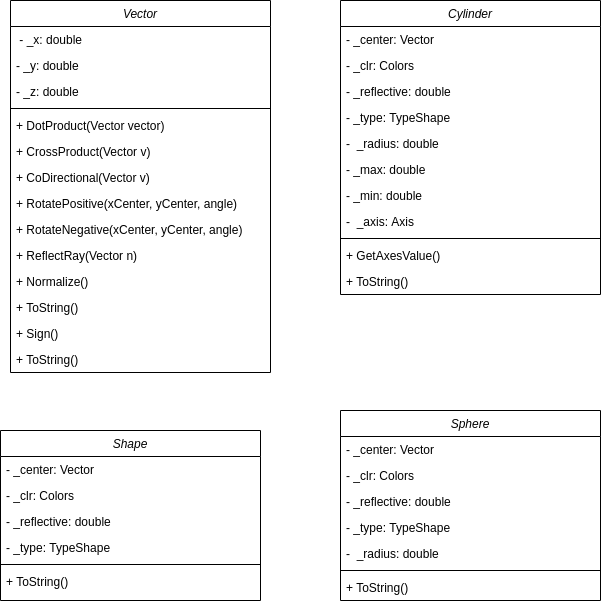
\includegraphics[width=0.8\textwidth]{class_diagram1.png}
		\caption{Структура классов}
		\label{fig:class_diagram1}}
\end{figure}

\begin{figure}[ht!]
	\centering{
		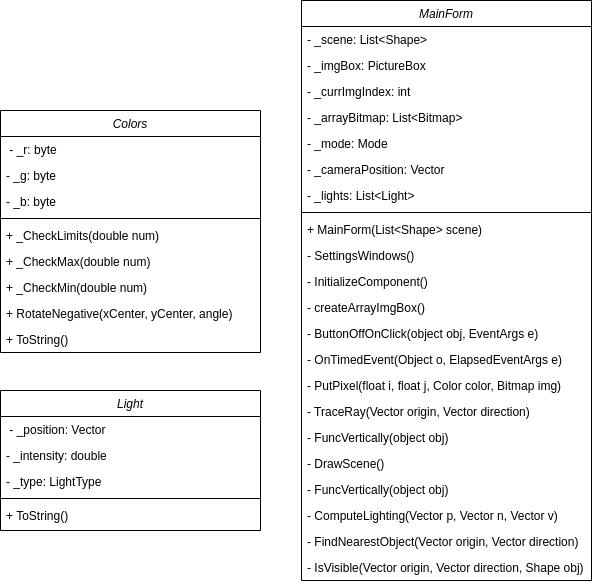
\includegraphics[width=0.8\textwidth]{class_diagram2.png}
		\caption{Структура классов}
		\label{fig:class_diagram2}}
\end{figure}

На листингах 3.1-3.2 представлен основной код программы.

\begin{lstlisting}[label=some-code,caption=Трассировка лучей.]
\end{lstlisting}

\section{Вывод}

В данном разделе были разобраны листинги рис 3.1-3.2, показывающие работу алгоритма.